\section{Construção e atualização de uma BITree}

\begin{frame}[fragile]{Atualização de um elemento}

    \begin{itemize}
        \item A árvore de Fenwick permite a atualização de um valor da sequência $a_k$ 
            original

        \item Para incrementar o elemento $a_i$ em $x$ unidades, é preciso adicionar $x$ em
             todos os intervalos onde este elemento é contabilizado

        \item A sequência dos intervalos $I_{k_1}, I_{k_2}, \ldots, I_{k_s}$, com $s = O(\log N)$,
            que contabilizam $a_i$, é tal que $k_1 = i$ e
        \[
            k_j = k_{j - 1} + p(k_{j - 1})
        \]

        \item A sequência é interrompida em $k_s$, onde $k_{s + 1} > N$

        \item Assim, a operação \code{c}{add(i, x)} tem complexidade $O(\log N)$
    \end{itemize}

\end{frame}

\begin{frame}[fragile]{Visualização de uma atualização em uma BITree}

    \begin{figure}
        \centering

        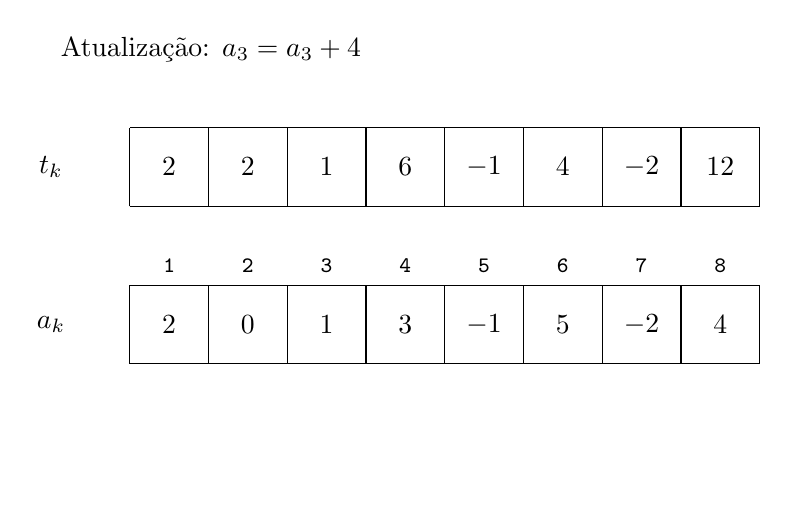
\begin{tikzpicture}
            \node[anchor=west] at (0, 12) { Atualização: $a_3 = a_3 + 4$ };

            \draw (1, 10) grid (9, 11);
            \draw (1, 8) grid (9, 9);

            \node at (0, 8.5) { $a_k$ };
            \node at (0, 10.5) { $t_k$ };

            \node[opacity=0, anchor=west] at (0, 6.5) { $r_1 = 3$ };

            \node at (1.5, 9.25) { \footnotesize \tt 1 };
            \node at (2.5, 9.25) { \footnotesize \tt 2 };
            \node at (3.5, 9.25) { \footnotesize \tt 3 };
            \node at (4.5, 9.25) { \footnotesize \tt 4 };
            \node at (5.5, 9.25) { \footnotesize \tt 5 };
            \node at (6.5, 9.25) { \footnotesize \tt 6 };
            \node at (7.5, 9.25) { \footnotesize \tt 7 };
            \node at (8.5, 9.25) { \footnotesize \tt 8 };

            \node at (1.5, 8.5) { \textcolor{black}{$2$} };
            \node at (2.5, 8.5) { \textcolor{black}{$0$} };
            \node at (3.5, 8.5) { \textcolor{black}{$1$} };
            \node at (4.5, 8.5) { \textcolor{black}{$3$} };
            \node at (5.5, 8.5) { \textcolor{black}{$-1$} };
            \node at (6.5, 8.5) { \textcolor{black}{$5$} };
            \node at (7.5, 8.5) { \textcolor{black}{$-2$} };
            \node at (8.5, 8.5) { \textcolor{black}{$4$} };

            \node at (1.5, 10.5) { \textcolor{black}{$2$} };
            \node at (2.5, 10.5) { \textcolor{black}{$2$} };
            \node at (3.5, 10.5) { \textcolor{black}{$1$} };
            \node at (4.5, 10.5) { \textcolor{black}{$6$} };
            \node at (5.5, 10.5) { \textcolor{black}{$-1$} };
            \node at (6.5, 10.5) { \textcolor{black}{$4$} };
            \node at (7.5, 10.5) { \textcolor{black}{$-2$} };
            \node at (8.5, 10.5) { \textcolor{black}{$12$} };

        \end{tikzpicture}

    \end{figure}

\end{frame}

\begin{frame}[fragile]{Visualização de uma atualização em uma BITree}

    \begin{figure}
        \centering

        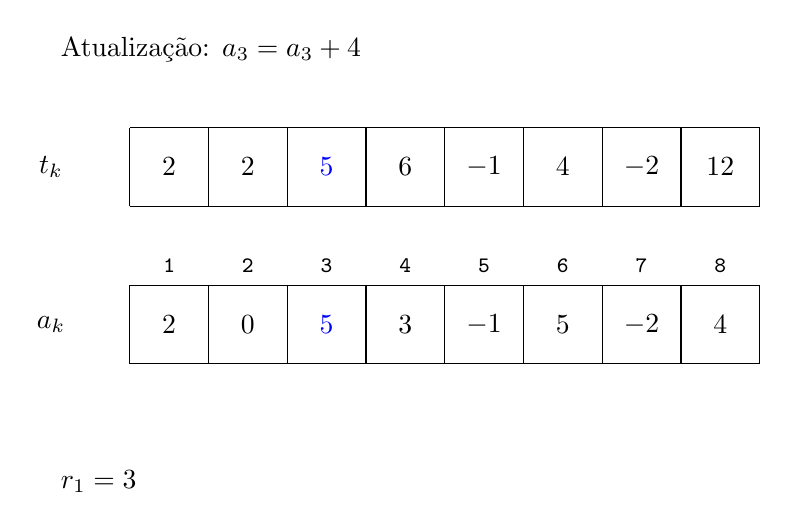
\begin{tikzpicture}
            \node[anchor=west] at (0, 12) { Atualização: $a_3 = a_3 + 4$ };

            \draw (1, 10) grid (9, 11);
            \draw (1, 8) grid (9, 9);

            \node at (0, 8.5) { $a_k$ };
            \node at (0, 10.5) { $t_k$ };

            \node[anchor=west] at (0, 6.5) { $r_1 = 3$ };

            \node at (1.5, 9.25) { \footnotesize \tt 1 };
            \node at (2.5, 9.25) { \footnotesize \tt 2 };
            \node at (3.5, 9.25) { \footnotesize \tt 3 };
            \node at (4.5, 9.25) { \footnotesize \tt 4 };
            \node at (5.5, 9.25) { \footnotesize \tt 5 };
            \node at (6.5, 9.25) { \footnotesize \tt 6 };
            \node at (7.5, 9.25) { \footnotesize \tt 7 };
            \node at (8.5, 9.25) { \footnotesize \tt 8 };

            \node at (1.5, 8.5) { \textcolor{black}{$2$} };
            \node at (2.5, 8.5) { \textcolor{black}{$0$} };
            \node at (3.5, 8.5) { \textcolor{blue}{$5$} };
            \node at (4.5, 8.5) { \textcolor{black}{$3$} };
            \node at (5.5, 8.5) { \textcolor{black}{$-1$} };
            \node at (6.5, 8.5) { \textcolor{black}{$5$} };
            \node at (7.5, 8.5) { \textcolor{black}{$-2$} };
            \node at (8.5, 8.5) { \textcolor{black}{$4$} };

            \node at (1.5, 10.5) { \textcolor{black}{$2$} };
            \node at (2.5, 10.5) { \textcolor{black}{$2$} };
            \node at (3.5, 10.5) { \textcolor{blue}{$5$} };
            \node at (4.5, 10.5) { \textcolor{black}{$6$} };
            \node at (5.5, 10.5) { \textcolor{black}{$-1$} };
            \node at (6.5, 10.5) { \textcolor{black}{$4$} };
            \node at (7.5, 10.5) { \textcolor{black}{$-2$} };
            \node at (8.5, 10.5) { \textcolor{black}{$12$} };

        \end{tikzpicture}

    \end{figure}

\end{frame}

\begin{frame}[fragile]{Visualização de uma atualização em uma BITree}

    \begin{figure}
        \centering

        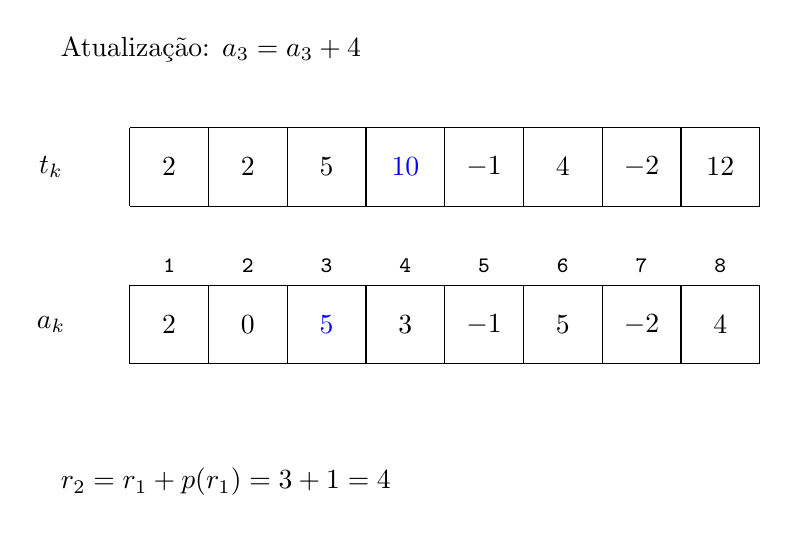
\begin{tikzpicture}
            \node[anchor=west] at (0, 12) { Atualização: $a_3 = a_3 + 4$ };

            \draw (1, 10) grid (9, 11);
            \draw (1, 8) grid (9, 9);

            \node at (0, 8.5) { $a_k$ };
            \node at (0, 10.5) { $t_k$ };

            \node[anchor=west] at (0, 6.5) { $r_2 = r_1 + p(r_1) = 3 + 1 = 4$ };

            \node at (1.5, 9.25) { \footnotesize \tt 1 };
            \node at (2.5, 9.25) { \footnotesize \tt 2 };
            \node at (3.5, 9.25) { \footnotesize \tt 3 };
            \node at (4.5, 9.25) { \footnotesize \tt 4 };
            \node at (5.5, 9.25) { \footnotesize \tt 5 };
            \node at (6.5, 9.25) { \footnotesize \tt 6 };
            \node at (7.5, 9.25) { \footnotesize \tt 7 };
            \node at (8.5, 9.25) { \footnotesize \tt 8 };

            \node at (1.5, 8.5) { \textcolor{black}{$2$} };
            \node at (2.5, 8.5) { \textcolor{black}{$0$} };
            \node at (3.5, 8.5) { \textcolor{blue}{$5$} };
            \node at (4.5, 8.5) { \textcolor{black}{$3$} };
            \node at (5.5, 8.5) { \textcolor{black}{$-1$} };
            \node at (6.5, 8.5) { \textcolor{black}{$5$} };
            \node at (7.5, 8.5) { \textcolor{black}{$-2$} };
            \node at (8.5, 8.5) { \textcolor{black}{$4$} };

            \node at (1.5, 10.5) { \textcolor{black}{$2$} };
            \node at (2.5, 10.5) { \textcolor{black}{$2$} };
            \node at (3.5, 10.5) { \textcolor{black}{$5$} };
            \node at (4.5, 10.5) { \textcolor{blue}{$10$} };
            \node at (5.5, 10.5) { \textcolor{black}{$-1$} };
            \node at (6.5, 10.5) { \textcolor{black}{$4$} };
            \node at (7.5, 10.5) { \textcolor{black}{$-2$} };
            \node at (8.5, 10.5) { \textcolor{black}{$12$} };

        \end{tikzpicture}

    \end{figure}

\end{frame}

\begin{frame}[fragile]{Visualização de uma atualização em uma BITree}

    \begin{figure}
        \centering

        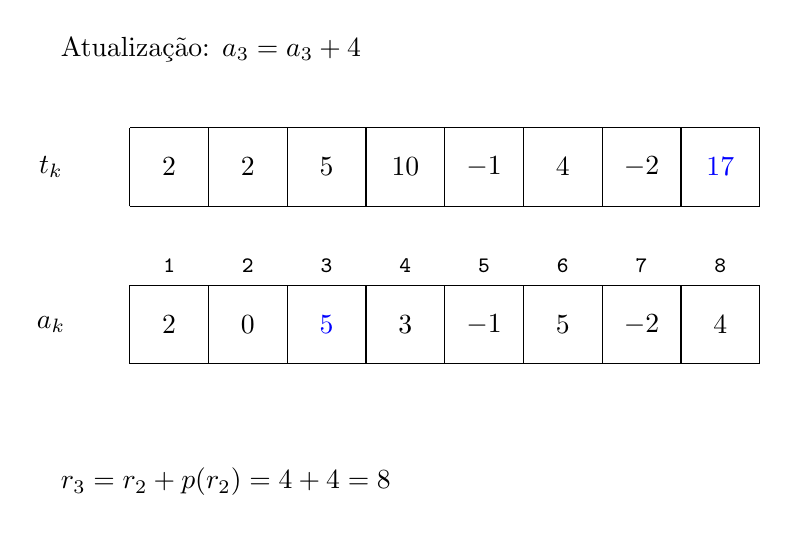
\begin{tikzpicture}
            \node[anchor=west] at (0, 12) { Atualização: $a_3 = a_3 + 4$ };

            \draw (1, 10) grid (9, 11);
            \draw (1, 8) grid (9, 9);

            \node at (0, 8.5) { $a_k$ };
            \node at (0, 10.5) { $t_k$ };

            \node[anchor=west] at (0, 6.5) { $r_3 = r_2 + p(r_2) = 4 + 4 = 8$ };

            \node at (1.5, 9.25) { \footnotesize \tt 1 };
            \node at (2.5, 9.25) { \footnotesize \tt 2 };
            \node at (3.5, 9.25) { \footnotesize \tt 3 };
            \node at (4.5, 9.25) { \footnotesize \tt 4 };
            \node at (5.5, 9.25) { \footnotesize \tt 5 };
            \node at (6.5, 9.25) { \footnotesize \tt 6 };
            \node at (7.5, 9.25) { \footnotesize \tt 7 };
            \node at (8.5, 9.25) { \footnotesize \tt 8 };

            \node at (1.5, 8.5) { \textcolor{black}{$2$} };
            \node at (2.5, 8.5) { \textcolor{black}{$0$} };
            \node at (3.5, 8.5) { \textcolor{blue}{$5$} };
            \node at (4.5, 8.5) { \textcolor{black}{$3$} };
            \node at (5.5, 8.5) { \textcolor{black}{$-1$} };
            \node at (6.5, 8.5) { \textcolor{black}{$5$} };
            \node at (7.5, 8.5) { \textcolor{black}{$-2$} };
            \node at (8.5, 8.5) { \textcolor{black}{$4$} };

            \node at (1.5, 10.5) { \textcolor{black}{$2$} };
            \node at (2.5, 10.5) { \textcolor{black}{$2$} };
            \node at (3.5, 10.5) { \textcolor{black}{$5$} };
            \node at (4.5, 10.5) { \textcolor{black}{$10$} };
            \node at (5.5, 10.5) { \textcolor{black}{$-1$} };
            \node at (6.5, 10.5) { \textcolor{black}{$4$} };
            \node at (7.5, 10.5) { \textcolor{black}{$-2$} };
            \node at (8.5, 10.5) { \textcolor{blue}{$17$} };

        \end{tikzpicture}

    \end{figure}

\end{frame}


\begin{frame}[fragile]{Implementação do método \code{c}{add(i, x)}}
    \inputsnippet{cpp}{35}{47}{codes/ft.cpp}
\end{frame}

\begin{frame}[fragile]{Construção de uma árvore de Fenwick}

    \begin{itemize}
        \item Uma maneira de se construir uma árvore de Fenwick é começar com um vetor cujos
            elementos são todos iguais a zero

        \item Depois, cada valor a ser atribuído à $i$-ésima posição deve ser somado a esta
            posição

        \item Como a operação de atualização/soma tem complexidade $O(\log N)$, onde $N$ é o 
            número máximo de elementos a serem inseridos na árvore, esta rotina tem complexidade
            $O(N\log N)$

    \end{itemize}

\end{frame}

\begin{frame}[fragile]{Visualização do construtor da árvore de segmentos}

    \begin{figure}
        \centering

        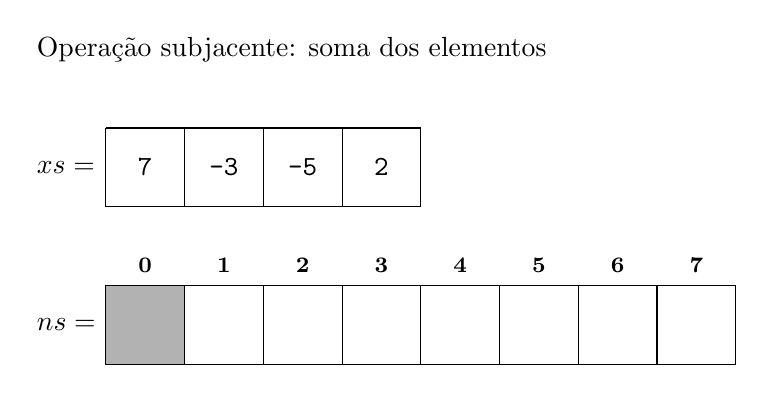
\begin{tikzpicture}
            \node[anchor=west] at (0, 5) { Operação subjacente: soma dos elementos };
            \node[anchor=west] at (0, 3.5) { $xs =$ };
            \node[anchor=west] at (0, 1.5) { $ns =$ };

            \draw[fill=gray!60] (1, 1) rectangle (2, 2);
            \draw (1, 3) grid (5, 4);
            \draw (1, 1) grid (9, 2);

            \node at (1.5, 2.25) { \footnotesize $\mathtt{\mathbf{0}}$ };
            \node at (2.5, 2.25) { \footnotesize $\mathtt{\mathbf{1}}$ };
            \node at (3.5, 2.25) { \footnotesize $\mathtt{\mathbf{2}}$ };
            \node at (4.5, 2.25) { \footnotesize $\mathtt{\mathbf{3}}$ };
            \node at (5.5, 2.25) { \footnotesize $\mathtt{\mathbf{4}}$ };
            \node at (6.5, 2.25) { \footnotesize $\mathtt{\mathbf{5}}$ };
            \node at (7.5, 2.25) { \footnotesize $\mathtt{\mathbf{6}}$ };
            \node at (8.5, 2.25) { \footnotesize $\mathtt{\mathbf{7}}$ };

            \node at (1.5, 3.5) { \tt 7 };
            \node at (2.5, 3.5) { \tt -3 };
            \node at (3.5, 3.5) { \tt -5 };
            \node at (4.5, 3.5) { \tt 2 };
        \end{tikzpicture}
    \end{figure}

\end{frame}

\begin{frame}[fragile]{Visualização do construtor da árvore de segmentos}

    \begin{figure}
        \centering

        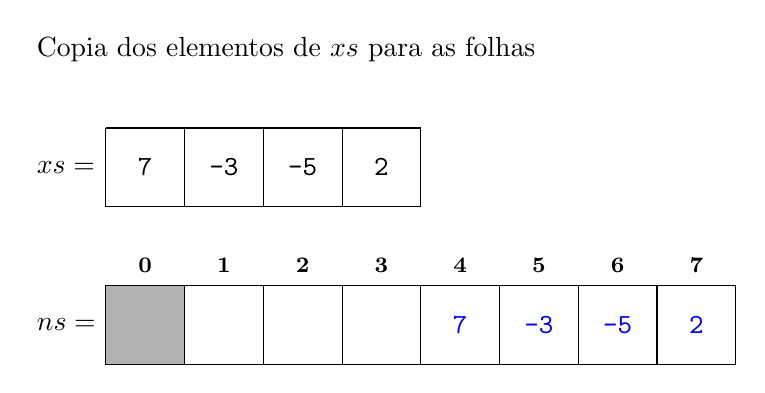
\begin{tikzpicture}
            \node[anchor=west] at (0, 5) { Copia dos elementos de $xs$ para as folhas };
            \node[anchor=west] at (0, 3.5) { $xs =$ };
            \node[anchor=west] at (0, 1.5) { $ns =$ };

            \draw[fill=gray!60] (1, 1) rectangle (2, 2);
            \draw (1, 3) grid (5, 4);
            \draw (1, 1) grid (9, 2);

            \node at (1.5, 2.25) { \footnotesize $\mathtt{\mathbf{0}}$ };
            \node at (2.5, 2.25) { \footnotesize $\mathtt{\mathbf{1}}$ };
            \node at (3.5, 2.25) { \footnotesize $\mathtt{\mathbf{2}}$ };
            \node at (4.5, 2.25) { \footnotesize $\mathtt{\mathbf{3}}$ };
            \node at (5.5, 2.25) { \footnotesize $\mathtt{\mathbf{4}}$ };
            \node at (6.5, 2.25) { \footnotesize $\mathtt{\mathbf{5}}$ };
            \node at (7.5, 2.25) { \footnotesize $\mathtt{\mathbf{6}}$ };
            \node at (8.5, 2.25) { \footnotesize $\mathtt{\mathbf{7}}$ };

            \node at (1.5, 3.5) { \tt 7 };
            \node at (2.5, 3.5) { \tt -3 };
            \node at (3.5, 3.5) { \tt -5 };
            \node at (4.5, 3.5) { \tt 2 };

            \node at (5.5, 1.5) { \tt \textcolor{blue}{7} };
            \node at (6.5, 1.5) { \tt \textcolor{blue}{-3} };
            \node at (7.5, 1.5) { \tt \textcolor{blue}{-5} };
            \node at (8.5, 1.5) { \tt \textcolor{blue}{2} };
        \end{tikzpicture}
    \end{figure}

\end{frame}

\begin{frame}[fragile]{Visualização do construtor da árvore de segmentos}

    \begin{figure}
        \centering

        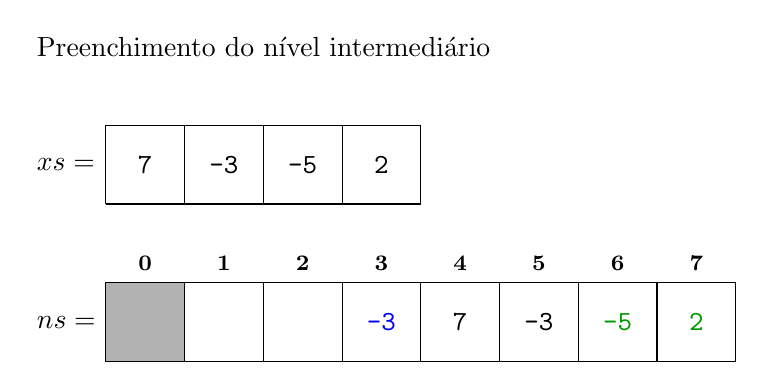
\begin{tikzpicture}
            \node[anchor=west] at (0, 5) { Preenchimento do nível intermediário };
            \node[anchor=west] at (0, 3.5) { $xs =$ };
            \node[anchor=west] at (0, 1.5) { $ns =$ };

            \draw[fill=gray!60] (1, 1) rectangle (2, 2);
            \draw (1, 3) grid (5, 4);
            \draw (1, 1) grid (9, 2);

            \node at (1.5, 2.25) { \footnotesize $\mathtt{\mathbf{0}}$ };
            \node at (2.5, 2.25) { \footnotesize $\mathtt{\mathbf{1}}$ };
            \node at (3.5, 2.25) { \footnotesize $\mathtt{\mathbf{2}}$ };
            \node at (4.5, 2.25) { \footnotesize $\mathtt{\mathbf{3}}$ };
            \node at (5.5, 2.25) { \footnotesize $\mathtt{\mathbf{4}}$ };
            \node at (6.5, 2.25) { \footnotesize $\mathtt{\mathbf{5}}$ };
            \node at (7.5, 2.25) { \footnotesize $\mathtt{\mathbf{6}}$ };
            \node at (8.5, 2.25) { \footnotesize $\mathtt{\mathbf{7}}$ };

            \node at (1.5, 3.5) { \tt 7 };
            \node at (2.5, 3.5) { \tt -3 };
            \node at (3.5, 3.5) { \tt -5 };
            \node at (4.5, 3.5) { \tt 2 };

            \node at (4.5, 1.5) { \tt \textcolor{blue}{-3} };
            \node at (5.5, 1.5) { \tt \textcolor{black}{7} };
            \node at (6.5, 1.5) { \tt \textcolor{black}{-3} };
            \node at (7.5, 1.5) { \tt \textcolor{green!60!black}{-5} };
            \node at (8.5, 1.5) { \tt \textcolor{green!60!black}{2} };
        \end{tikzpicture}
    \end{figure}

\end{frame}

\begin{frame}[fragile]{Visualização do construtor da árvore de segmentos}

    \begin{figure}
        \centering

        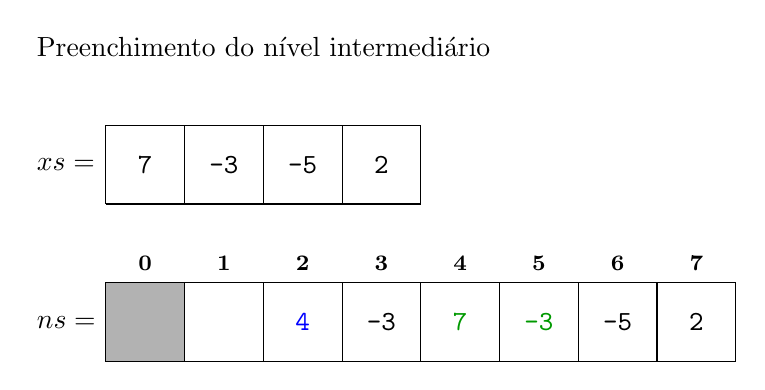
\begin{tikzpicture}
            \node[anchor=west] at (0, 5) { Preenchimento do nível intermediário };
            \node[anchor=west] at (0, 3.5) { $xs =$ };
            \node[anchor=west] at (0, 1.5) { $ns =$ };

            \draw[fill=gray!60] (1, 1) rectangle (2, 2);
            \draw (1, 3) grid (5, 4);
            \draw (1, 1) grid (9, 2);

            \node at (1.5, 2.25) { \footnotesize $\mathtt{\mathbf{0}}$ };
            \node at (2.5, 2.25) { \footnotesize $\mathtt{\mathbf{1}}$ };
            \node at (3.5, 2.25) { \footnotesize $\mathtt{\mathbf{2}}$ };
            \node at (4.5, 2.25) { \footnotesize $\mathtt{\mathbf{3}}$ };
            \node at (5.5, 2.25) { \footnotesize $\mathtt{\mathbf{4}}$ };
            \node at (6.5, 2.25) { \footnotesize $\mathtt{\mathbf{5}}$ };
            \node at (7.5, 2.25) { \footnotesize $\mathtt{\mathbf{6}}$ };
            \node at (8.5, 2.25) { \footnotesize $\mathtt{\mathbf{7}}$ };

            \node at (1.5, 3.5) { \tt 7 };
            \node at (2.5, 3.5) { \tt -3 };
            \node at (3.5, 3.5) { \tt -5 };
            \node at (4.5, 3.5) { \tt 2 };

            \node at (3.5, 1.5) { \tt \textcolor{blue}{4} };
            \node at (4.5, 1.5) { \tt \textcolor{black}{-3} };
            \node at (5.5, 1.5) { \tt \textcolor{green!60!black}{7} };
            \node at (6.5, 1.5) { \tt \textcolor{green!60!black}{-3} };
            \node at (7.5, 1.5) { \tt \textcolor{black}{-5} };
            \node at (8.5, 1.5) { \tt \textcolor{black}{2} };
        \end{tikzpicture}
    \end{figure}

\end{frame}

\begin{frame}[fragile]{Visualização do construtor da árvore de segmentos}

    \begin{figure}
        \centering

        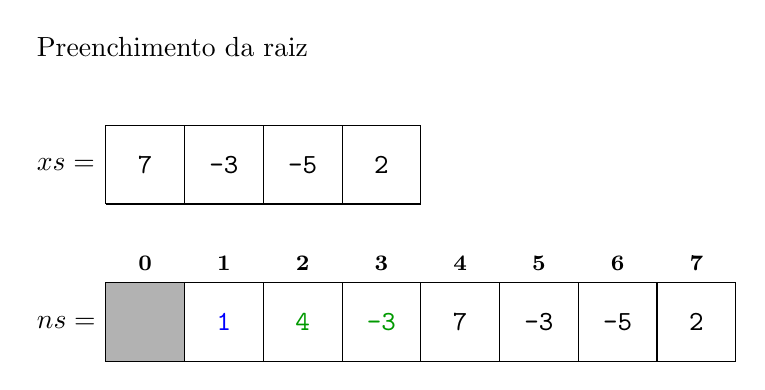
\begin{tikzpicture}
            \node[anchor=west] at (0, 5) { Preenchimento da raiz };
            \node[anchor=west] at (0, 3.5) { $xs =$ };
            \node[anchor=west] at (0, 1.5) { $ns =$ };

            \draw[fill=gray!60] (1, 1) rectangle (2, 2);
            \draw (1, 3) grid (5, 4);
            \draw (1, 1) grid (9, 2);

            \node at (1.5, 2.25) { \footnotesize $\mathtt{\mathbf{0}}$ };
            \node at (2.5, 2.25) { \footnotesize $\mathtt{\mathbf{1}}$ };
            \node at (3.5, 2.25) { \footnotesize $\mathtt{\mathbf{2}}$ };
            \node at (4.5, 2.25) { \footnotesize $\mathtt{\mathbf{3}}$ };
            \node at (5.5, 2.25) { \footnotesize $\mathtt{\mathbf{4}}$ };
            \node at (6.5, 2.25) { \footnotesize $\mathtt{\mathbf{5}}$ };
            \node at (7.5, 2.25) { \footnotesize $\mathtt{\mathbf{6}}$ };
            \node at (8.5, 2.25) { \footnotesize $\mathtt{\mathbf{7}}$ };

            \node at (1.5, 3.5) { \tt 7 };
            \node at (2.5, 3.5) { \tt -3 };
            \node at (3.5, 3.5) { \tt -5 };
            \node at (4.5, 3.5) { \tt 2 };

            \node at (2.5, 1.5) { \tt \textcolor{blue}{1} };
            \node at (3.5, 1.5) { \tt \textcolor{green!60!black}{4} };
            \node at (4.5, 1.5) { \tt \textcolor{green!60!black}{-3} };
            \node at (5.5, 1.5) { \tt \textcolor{black}{7} };
            \node at (6.5, 1.5) { \tt \textcolor{black}{-3} };
            \node at (7.5, 1.5) { \tt \textcolor{black}{-5} };
            \node at (8.5, 1.5) { \tt \textcolor{black}{2} };
        \end{tikzpicture}
    \end{figure}

\end{frame}

